\documentclass[12pt,a4paper]{article}
\usepackage{ctex}
\usepackage{amsmath,amscd,amsbsy,amssymb,latexsym,url,bm,amsthm}
\usepackage{epsfig,graphicx,subfigure}
\usepackage{enumitem,balance}
\usepackage{wrapfig}
\usepackage{mathrsfs,euscript}
\usepackage[usenames]{xcolor}
\usepackage{hyperref}
\usepackage[vlined,ruled,linesnumbered]{algorithm2e}
\hypersetup{colorlinks=true,linkcolor=black}

\newtheorem{theorem}{Theorem}
\newtheorem{lemma}[theorem]{Lemma}
\newtheorem{proposition}[theorem]{Proposition}
\newtheorem{corollary}[theorem]{Corollary}
\newtheorem{exercise}{Exercise}
\newtheorem*{solution}{Solution}
\newtheorem{definition}{Definition}
\theoremstyle{definition}

\renewcommand{\thefootnote}{\fnsymbol{footnote}}

\newcommand{\postscript}[2]
 {\setlength{\epsfxsize}{#2\hsize}
  \centerline{\epsfbox{#1}}}

\renewcommand{\baselinestretch}{1.0}

\setlength{\oddsidemargin}{-0.365in}
\setlength{\evensidemargin}{-0.365in}
\setlength{\topmargin}{-0.3in}
\setlength{\headheight}{0in}
\setlength{\headsep}{0in}
\setlength{\textheight}{10.1in}
\setlength{\textwidth}{7in}
\makeatletter \renewenvironment{proof}[1][Proof] {\par\pushQED{\qed}\normalfont\topsep6\p@\@plus6\p@\relax\trivlist\item[\hskip\labelsep\bfseries#1\@addpunct{.}]\ignorespaces}{\popQED\endtrivlist\@endpefalse} \makeatother
\makeatletter
\renewenvironment{solution}[1][Solution] {\par\pushQED{\qed}\normalfont\topsep6\p@\@plus6\p@\relax\trivlist\item[\hskip\labelsep\bfseries#1\@addpunct{.}]\ignorespaces}{\popQED\endtrivlist\@endpefalse} \makeatother

\begin{document}

\noindent

%========================================================================
\noindent\framebox[\linewidth]{\shortstack[c]{
\Large{\textbf{Lab08-Graph Exploration}}\vspace{1mm}\\
CS214-Algorithm and Complexity, Xiaofeng Gao, Spring 2020.}}
\begin{center}
\footnotesize{\color{red}$*$ If there is any problem, please contact TA Yiming Liu.}

% Please write down your name, student id and email.
\footnotesize{\color{blue}$*$ Name: Futao Wei  \quad Student ID: 518021910750 \quad Email: weifutao@sjtu.edu.cn}
\end{center}

\begin{enumerate}
    \item
    \textbf{BFS Tree.} Similar to DFS, BFS yields a tree, (also possibly forest, but \textbf{just consider a tree} in this question) and we can define \textbf{tree, forward, back, cross} edges for BFS. Denote $Dist(u)$ as the distance between node $u$ and the source node in the BFS tree. Please prove:
    \begin{enumerate}
    	\item For both undirected and directed graphs, no forward edges exist in the graph.
    	
    	\item There are no back edges in undirected graph, while in directed graph each back edge $(u,v)$ yields $0\leq Dist(v)\leq Dist(u)$.
    	
    	\item For undirected graph, each cross edge $(u,v)$ yields $|Dist(v)-Dist(u)|\le 1$, while for directed graph, each cross edge $(u,v)$ yields $Dist(v)\leq Dist(u)+1$.
    	
    \end{enumerate}
	
	\begin{solution}
		\hfill
		\begin{enumerate}
			\item 
			Suppose for contradiction that $(u, v)$ is a forward edge in the graph, and that $t$ is $u$'s child as well as $v$'s ancestor in the BFS tree. Then $v$ should be $u$'s child in the BFS tree --- a contradiction! 
			\item
			The undirected case can be proved as in (a). \\
			According to the definition of the back edge, $v$ is an ancestor of $u$ in the BFS tree. Hence it's obvious that $0\leq Dist(v)\leq Dist(u)$.
			\item
			For undirected graph, assume for contradiction that some cross edge $(u, v)$ yields $|Dist(v)-Dist(u)|\geq 2$. Then we get a contradiction that $(u, v)$ cannot be a cross edge, since $u$ would have been a child of $v$ or vice versa. \\
			For directed graph, suppose for contradiction that some cross edge $(u, v)$ yields $Dist(v)\geq Dist(u)+2$. Then we have a contradiction that $(u, v)$ cannot be a cross edge, since $v$ would have been a child of $u$.
		\end{enumerate}
	\end{solution}

    \item 
    \textbf{Articulation Points, Bridges, and Biconnected Components.} Let $G=(V, E)$ be a connected, undirected graph. An articulation point of $G$ is a vertex whose removal disconnects $G$. A bridge of $G$ is an edge whose removal disconnects $G .$ A biconnected component of $G$ is a maximal set of edges such that any two edges in the set lie on a common simple cycle. Figure\ref{def} illustrates these definitions. We can determine articulation points, bridges, and biconnected components using depth-first search. Let $G_{\pi}=\left(V, E_{\pi}\right)$ be a depth-first tree of $G$. Please prove:
    
    \begin{enumerate}
    	\item The root of $G_{\pi}$ is an articulation point of $G$ if and only if it has at least two children in $G_{\pi}$.
    	\item An edge of $G$ is a bridge if and only if it does not lie on any simple cycle of $G$.
    	\item The biconnected components of $G$ partition the nonbridge edges of $G$.
    \end{enumerate}

	 \begin{figure}[htbp]
	 	
		\centering
		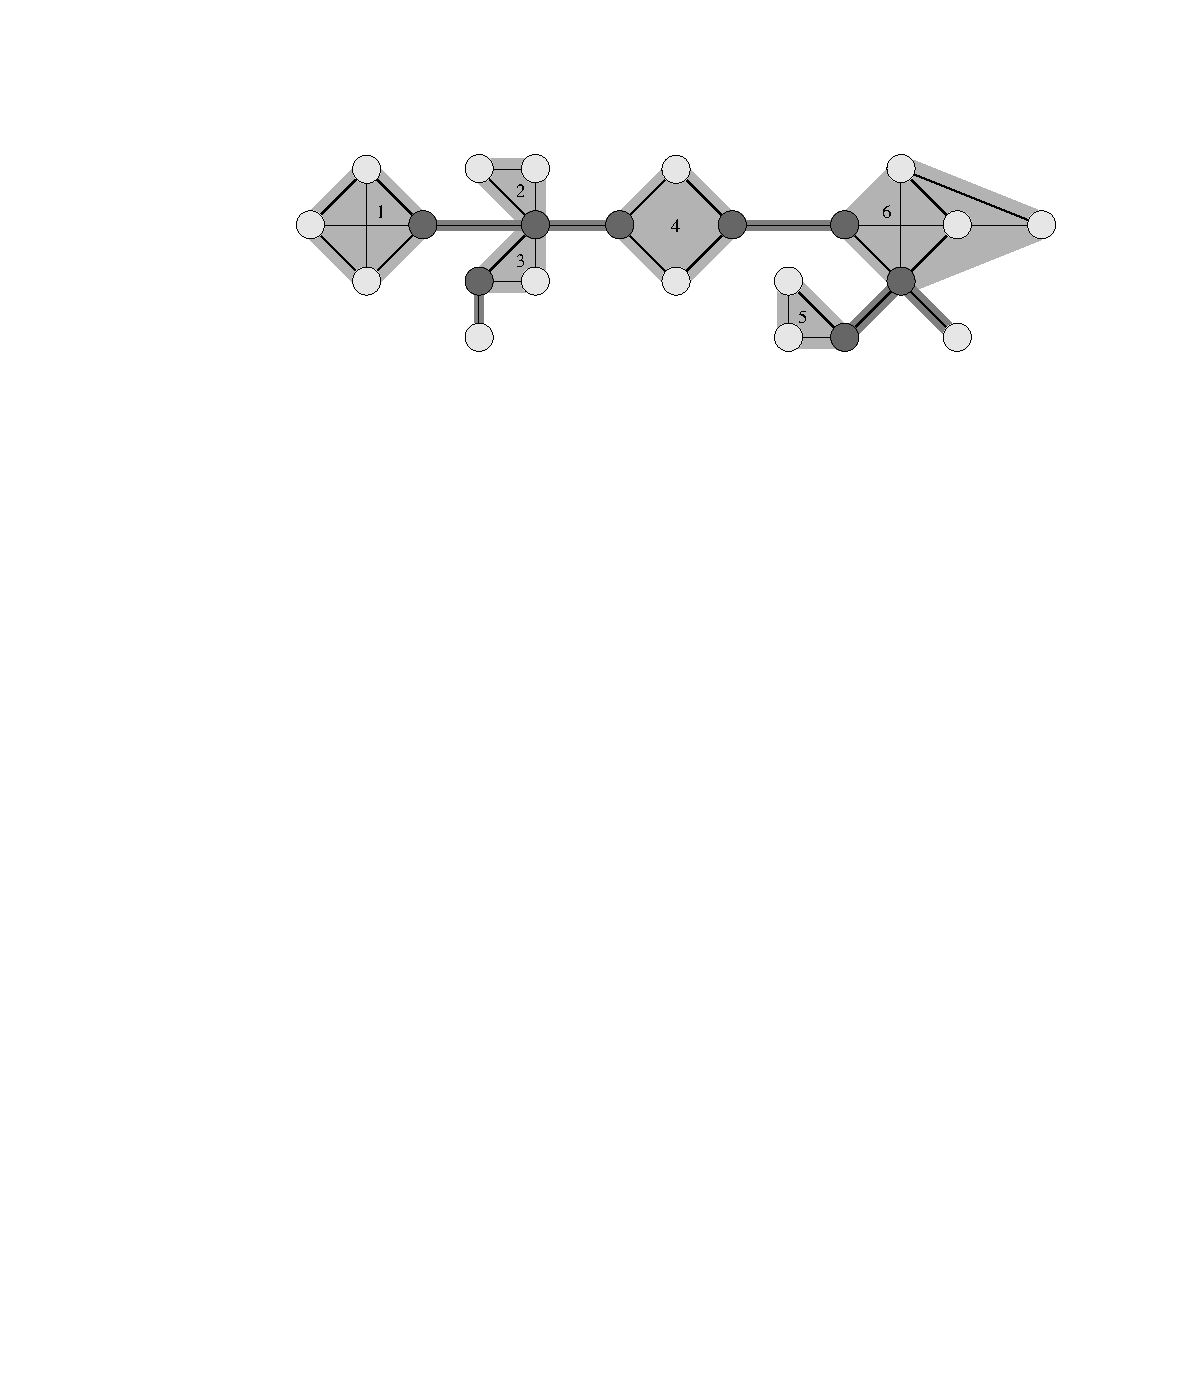
\includegraphics[width=6in]{Fig-Definition.pdf}
		\caption{The definition of articulation points, bridges, and biconnected components. The articulation points are the heavily shaded vertices, the bridges are the heavily shaded edges, and the biconnected components are the edges in the shaded regions, with a \textit{bcc} numbering shown.}
		\label{def}
	\end{figure}
	
	\begin{solution}
		\hfill
		\begin{enumerate}
			\item 
			$\implies$: \\
			Suppose for contradiction that the root of $G_{\pi}$ has only one child. Then its removal does not disconnect $G$, i.e., it's not an articulation point of $G$ --- a contradiction! \\
			$\impliedby$: Trivial.
			\item
			$\implies$: \\
			Suppose for contradiction that a bridge edge of $G$ lies on some simple cycle of $G$. Then its removal will not disconnect $G$ --- a contradiction! \\
			$\impliedby$: Trivial.
			\item
			The biconnected components of $G$ partition the nonbridge edges of $G$. $\iff$ Any of the non-bridge edges in $G$ is in only one biconnected component of $G$. \\
			The contrapositive of (b) shows that any non-bridge edge of $G$ lies on some simple cycle of $G$, i.e., on at least one biconnected component. \\
			Suppose that some non-bridge edge of $G$ lies on two biconnected components. Then the combination of the two components is actually a larger biconnected component. Hence any non-bridge edge of $G$ is in only one biconnected component of $G$. 
		\end{enumerate}
	\end{solution}
    \item
    Suppose $G=(V, E)$ is a \textbf{Directed Acyclic Graph} (DAG) with positive weights $w(u, v)$ on each edge. Let $s$ be a vertex of $G$ with no incoming edges and assume that every other node is reachable from $s$ through some path.
    
    \begin{enumerate}
    	\item
    	Give an $O(|V|+|E|)$-time algorithm to compute the shortest paths from $s$ to all the other vertices in $G$. Note that this is faster than Dijkstra's algorithm in general.
    	\item
    	Give an efficient algorithm to compute the longest paths from $s$ to all the other vertices.
    \end{enumerate}
    \begin{solution}
    	\hfill
    	\begin{enumerate}
    		\item 
    		\begin{minipage}[t]{0.9\textwidth}
    			\begin{algorithm}[H]
    				\caption{Sort$(G, s)$}
    				\KwIn{$G=(V,E)$, vertex $s \in V$, $stack = \emptyset$}
    				\KwOut{$stack$}
    				$visited[s] = True$\;
    				\ForEach{$(s, v) \in E$}{
    					\If{$not \, visited[v]$}{
    						Sort$(G,v)$\;
    					}
    				}
    				$stack$.push$(s)$\;
    				\textbf{return} $stack$\;
    			\end{algorithm}
    			\begin{algorithm}[H]
    				\caption{SP$(G,s)$}
    				\KwIn{$G=(V,E), s$}
    				\KwOut{$dist[1, \cdots , n]$}
    				\For{$i = 1 \textbf{ to } n$}{
    					$dist[i] = \infty$\;
    				}
    				$stack =$ Sort$(G, s)$\;
    				\While{$not \, stack$.empty()}{
    					$v = stack$.pop()\;
    					\ForEach{$(v, u) \in E$}{
    						\If{$dist[u] > dist[v] + w(v, u)$}{
    							$dist[u] = dist[v] + w(v, u)$\;
    						}
    					}
    				}
    				\textbf{return} $dist[1, \cdots , n]$\;
    			\end{algorithm}
    		\end{minipage}
    		This algorithm is very similar to Dijkstra's algorithm except for using a stack rather than a heap. Hence it's faster than Dijkstra's algorithm.
    		\item
    		\begin{minipage}[t]{0.9\textwidth}
    			\begin{algorithm}[H]
    				\caption{LP$(G,s)$}
    				\KwIn{$G=(V,E), s$}
    				\KwOut{$dist[1, \cdots , n]$}
    				\For{$i = 1 \textbf{ to } n$}{
    					$dist[i] = 0$\;
    				}
    				$stack =$ Sort$(G, s)$\;
    				\While{$not \, stack$.empty()}{
    					$v = stack$.pop()\;
    					\ForEach{$(v, u) \in E$}{
    						\If{$dist[u] < dist[v] + w(v, u)$}{
    							$dist[u] = dist[v] + w(v, u)$\;
    						}
    					}
    				}
    				\textbf{return} $dist[1, \cdots , n]$\;
    			\end{algorithm}
    		\end{minipage}
    	\end{enumerate}
    \end{solution}
\end{enumerate}

\vspace{20pt}

\textbf{Remark:} You need to include your .pdf and .tex files in your uploaded .rar or .zip file.

%========================================================================
\end{document}
